\section{Model Serving}\label{chap:model-serving}

Dalam tugas akhir ini akan dibahas secara lebih mendalam terkait Model Serving.
Hal-hal yang akan dibahas meliputi metode-metode yang ada dalam melakukan \textit{serving} dan teknologi apa saja yang digunakan untuk membangun arsitektur \textit{deployment} model tersebut.

Terdapat lima jenis \textit{serving pattern} yang umum digunakan untuk membuat layanan dari model (\cite{mlopsorg}):
\begin{enumerate}
  \item Model-as-Service
  \item Model-as-Dependency
  \item Precompute Serving
  \item Model-on-Demand
  \item Hybrid Serving
\end{enumerate}

\subsection{Model-as-Service}

\begin{figure}[ht]
  \centering
  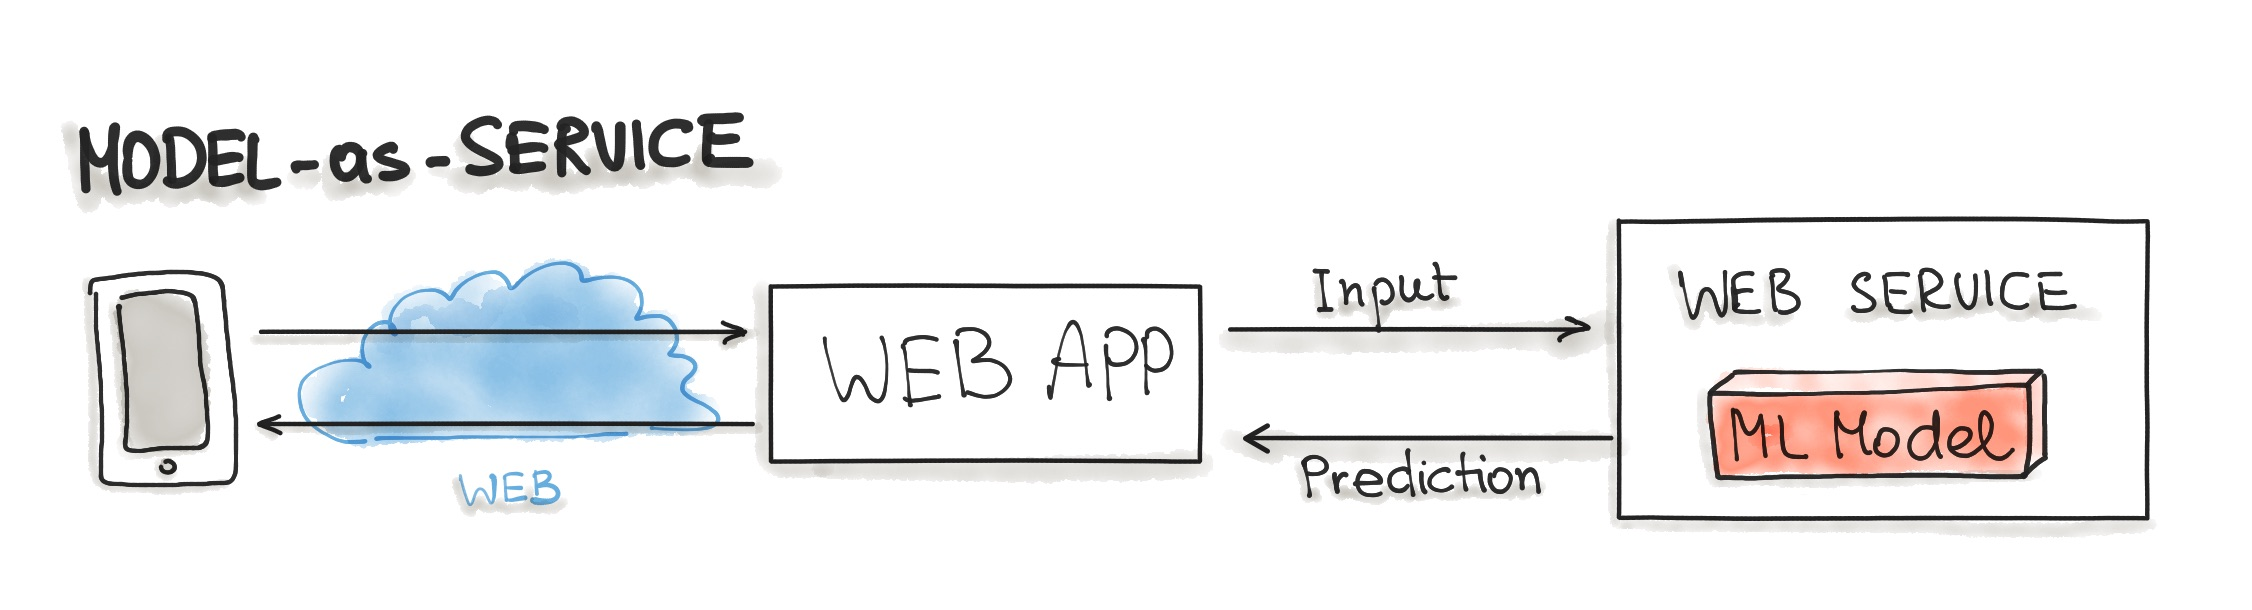
\includegraphics[width=0.7\textwidth]{02-model-as-service.jpg}
  \caption{Ilustrasi Model-as-Service (Sumber:~\cite{book-handsonml})}\label{fig:model-as-service}
\end{figure}

\textit{Serving pattern} ini adalah metode yang paling sederhana.
Pada dasarnya, model yang sudah ada akan dibungkus dengan sebuah \textit{interface} agar dapat dilakukan RPC terhadap model tersebut (lihat Gambar~\ref{fig:model-as-service}).
Teknologi yang umum digunakan biasanya seperti REST API dan gRPC, namun metode-metode RPC lainnya dapat juga digunakan.

\subsection{Model-as-Dependency}

\begin{figure}[ht]
  \centering
  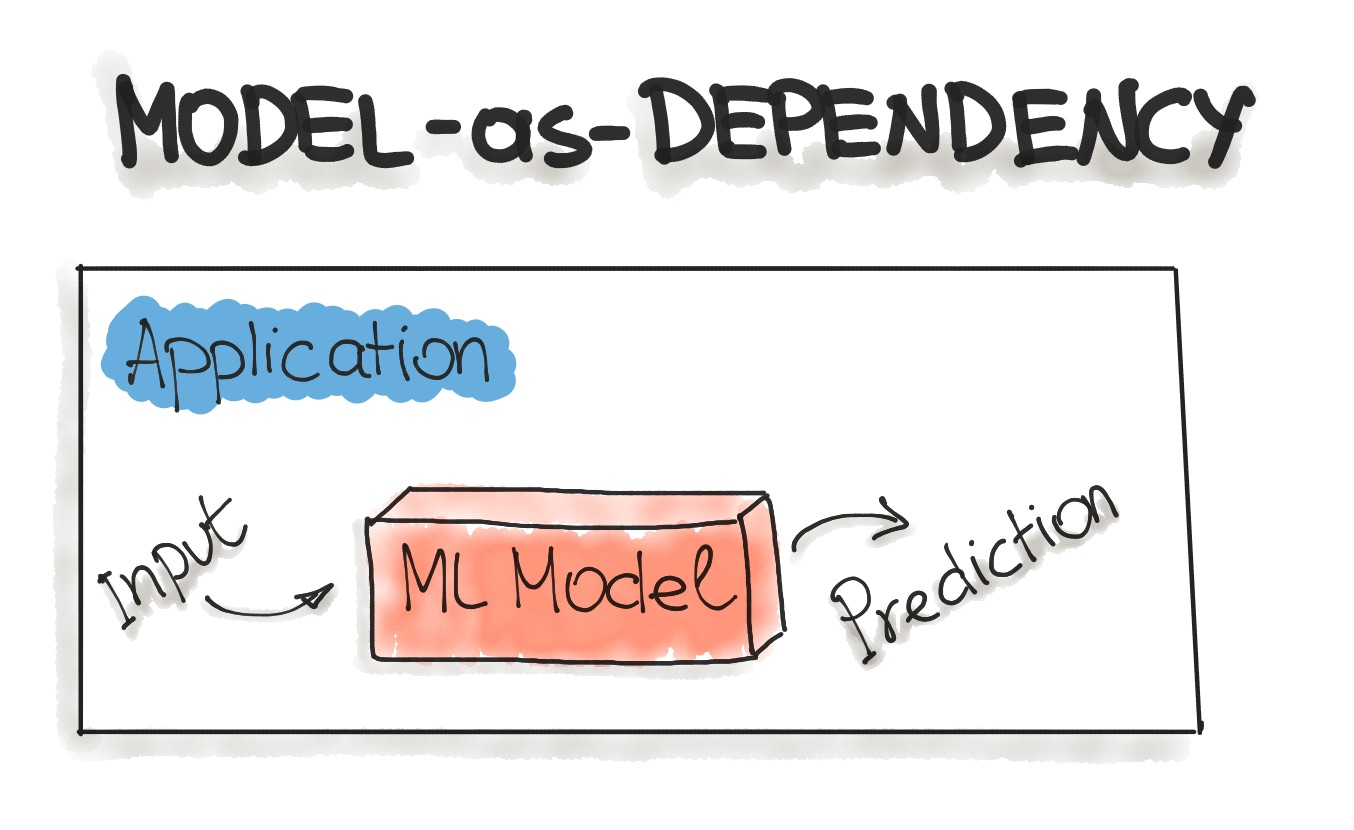
\includegraphics[width=0.7\textwidth]{02-model-as-dependency.jpg}
  \caption{Ilustrasi Model-as-Dependency (Sumber:~\cite{book-handsonml})}\label{fig:model-as-dependency}
\end{figure}

\textit{Serving pattern} serupa dengan Model-as-Service, dengan pembeda utamanya adalah model tersebut menjadi \textit{dependency} dari layanan yang dibuat secara internal, bukan melakukan \textit{deployment} secara terpisah untuk model tersebut (lihat Gambar~\ref{fig:model-as-dependency}).
\textit{Pattern} ini akan digunakan apabila model akan digunakan sebagai satu bagian dari layanan yang lebih besar.

\subsection{Precompute Serving}

\begin{figure}[ht]
  \centering
  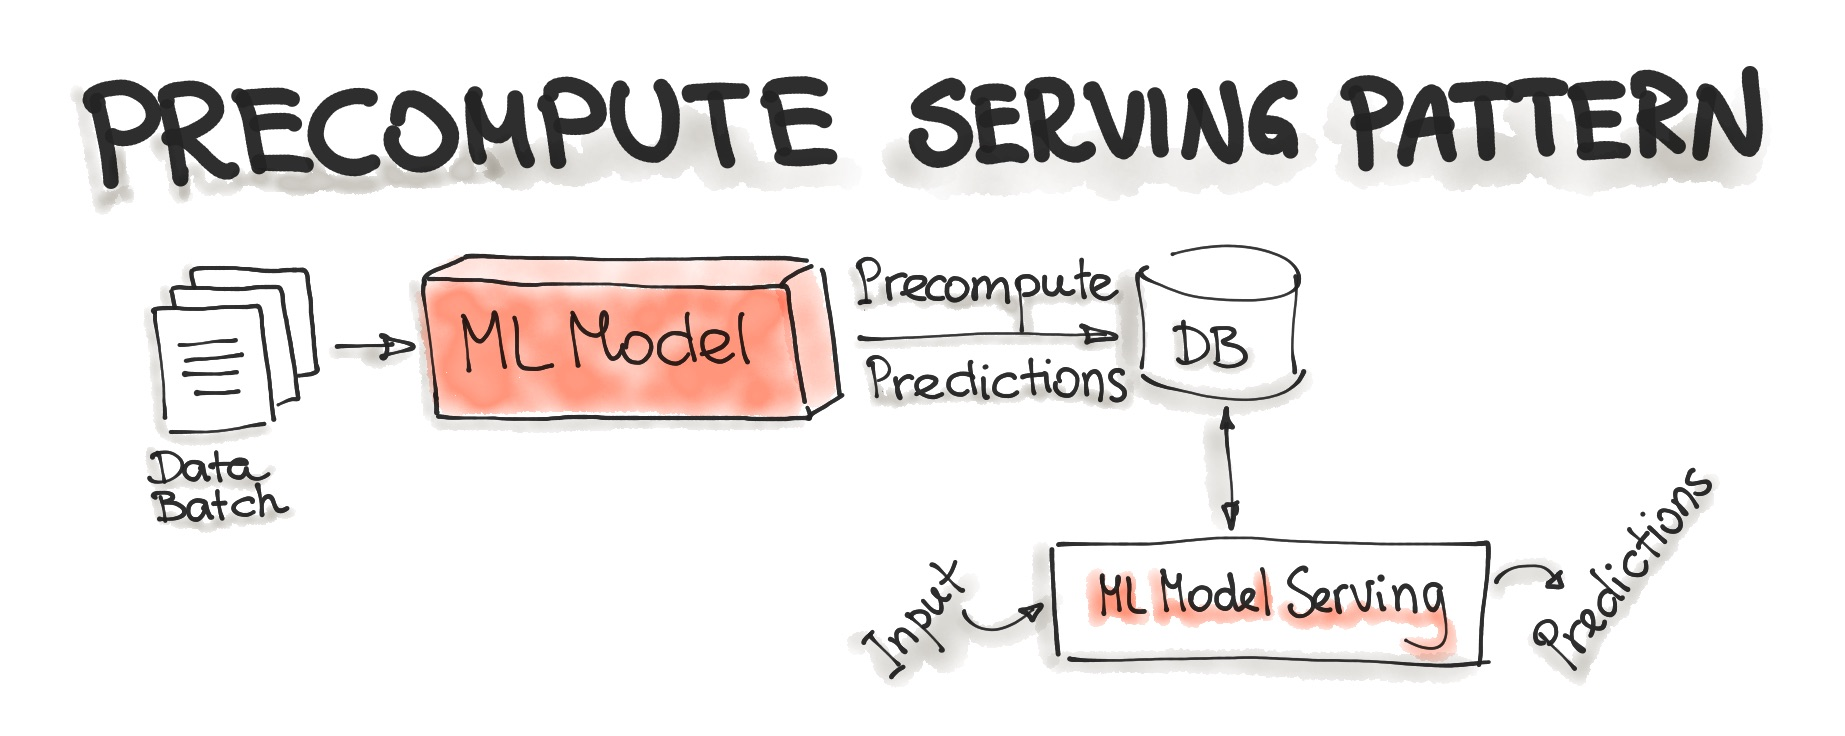
\includegraphics[width=0.7\textwidth]{02-precompute-serving-pattern.jpg}
  \caption{Ilustrasi Precompute Serving Pattern (Sumber:~\cite{book-handsonml})}\label{fig:precompute-serving}
\end{figure}

Sesuai namanya, model akan digunakan untuk melakukan prekomputasi tanpa langsung menggunakan modelnya dalam sistem (lihat Gambar~\ref{fig:precompute-serving}).
Hasil dari prekomputasi yang dilakukan biasanya akan disimpan pada suatu basis data, yang nantinya akan digunakan oleh layanan tertentu.
Model tidak perlu dijalankan terus menerus, melainkan hanya perlu dijalankan bila diperlukan atau secara berkala saja.

\subsection{Model-on-Demand}

\begin{figure}[ht]
  \centering
  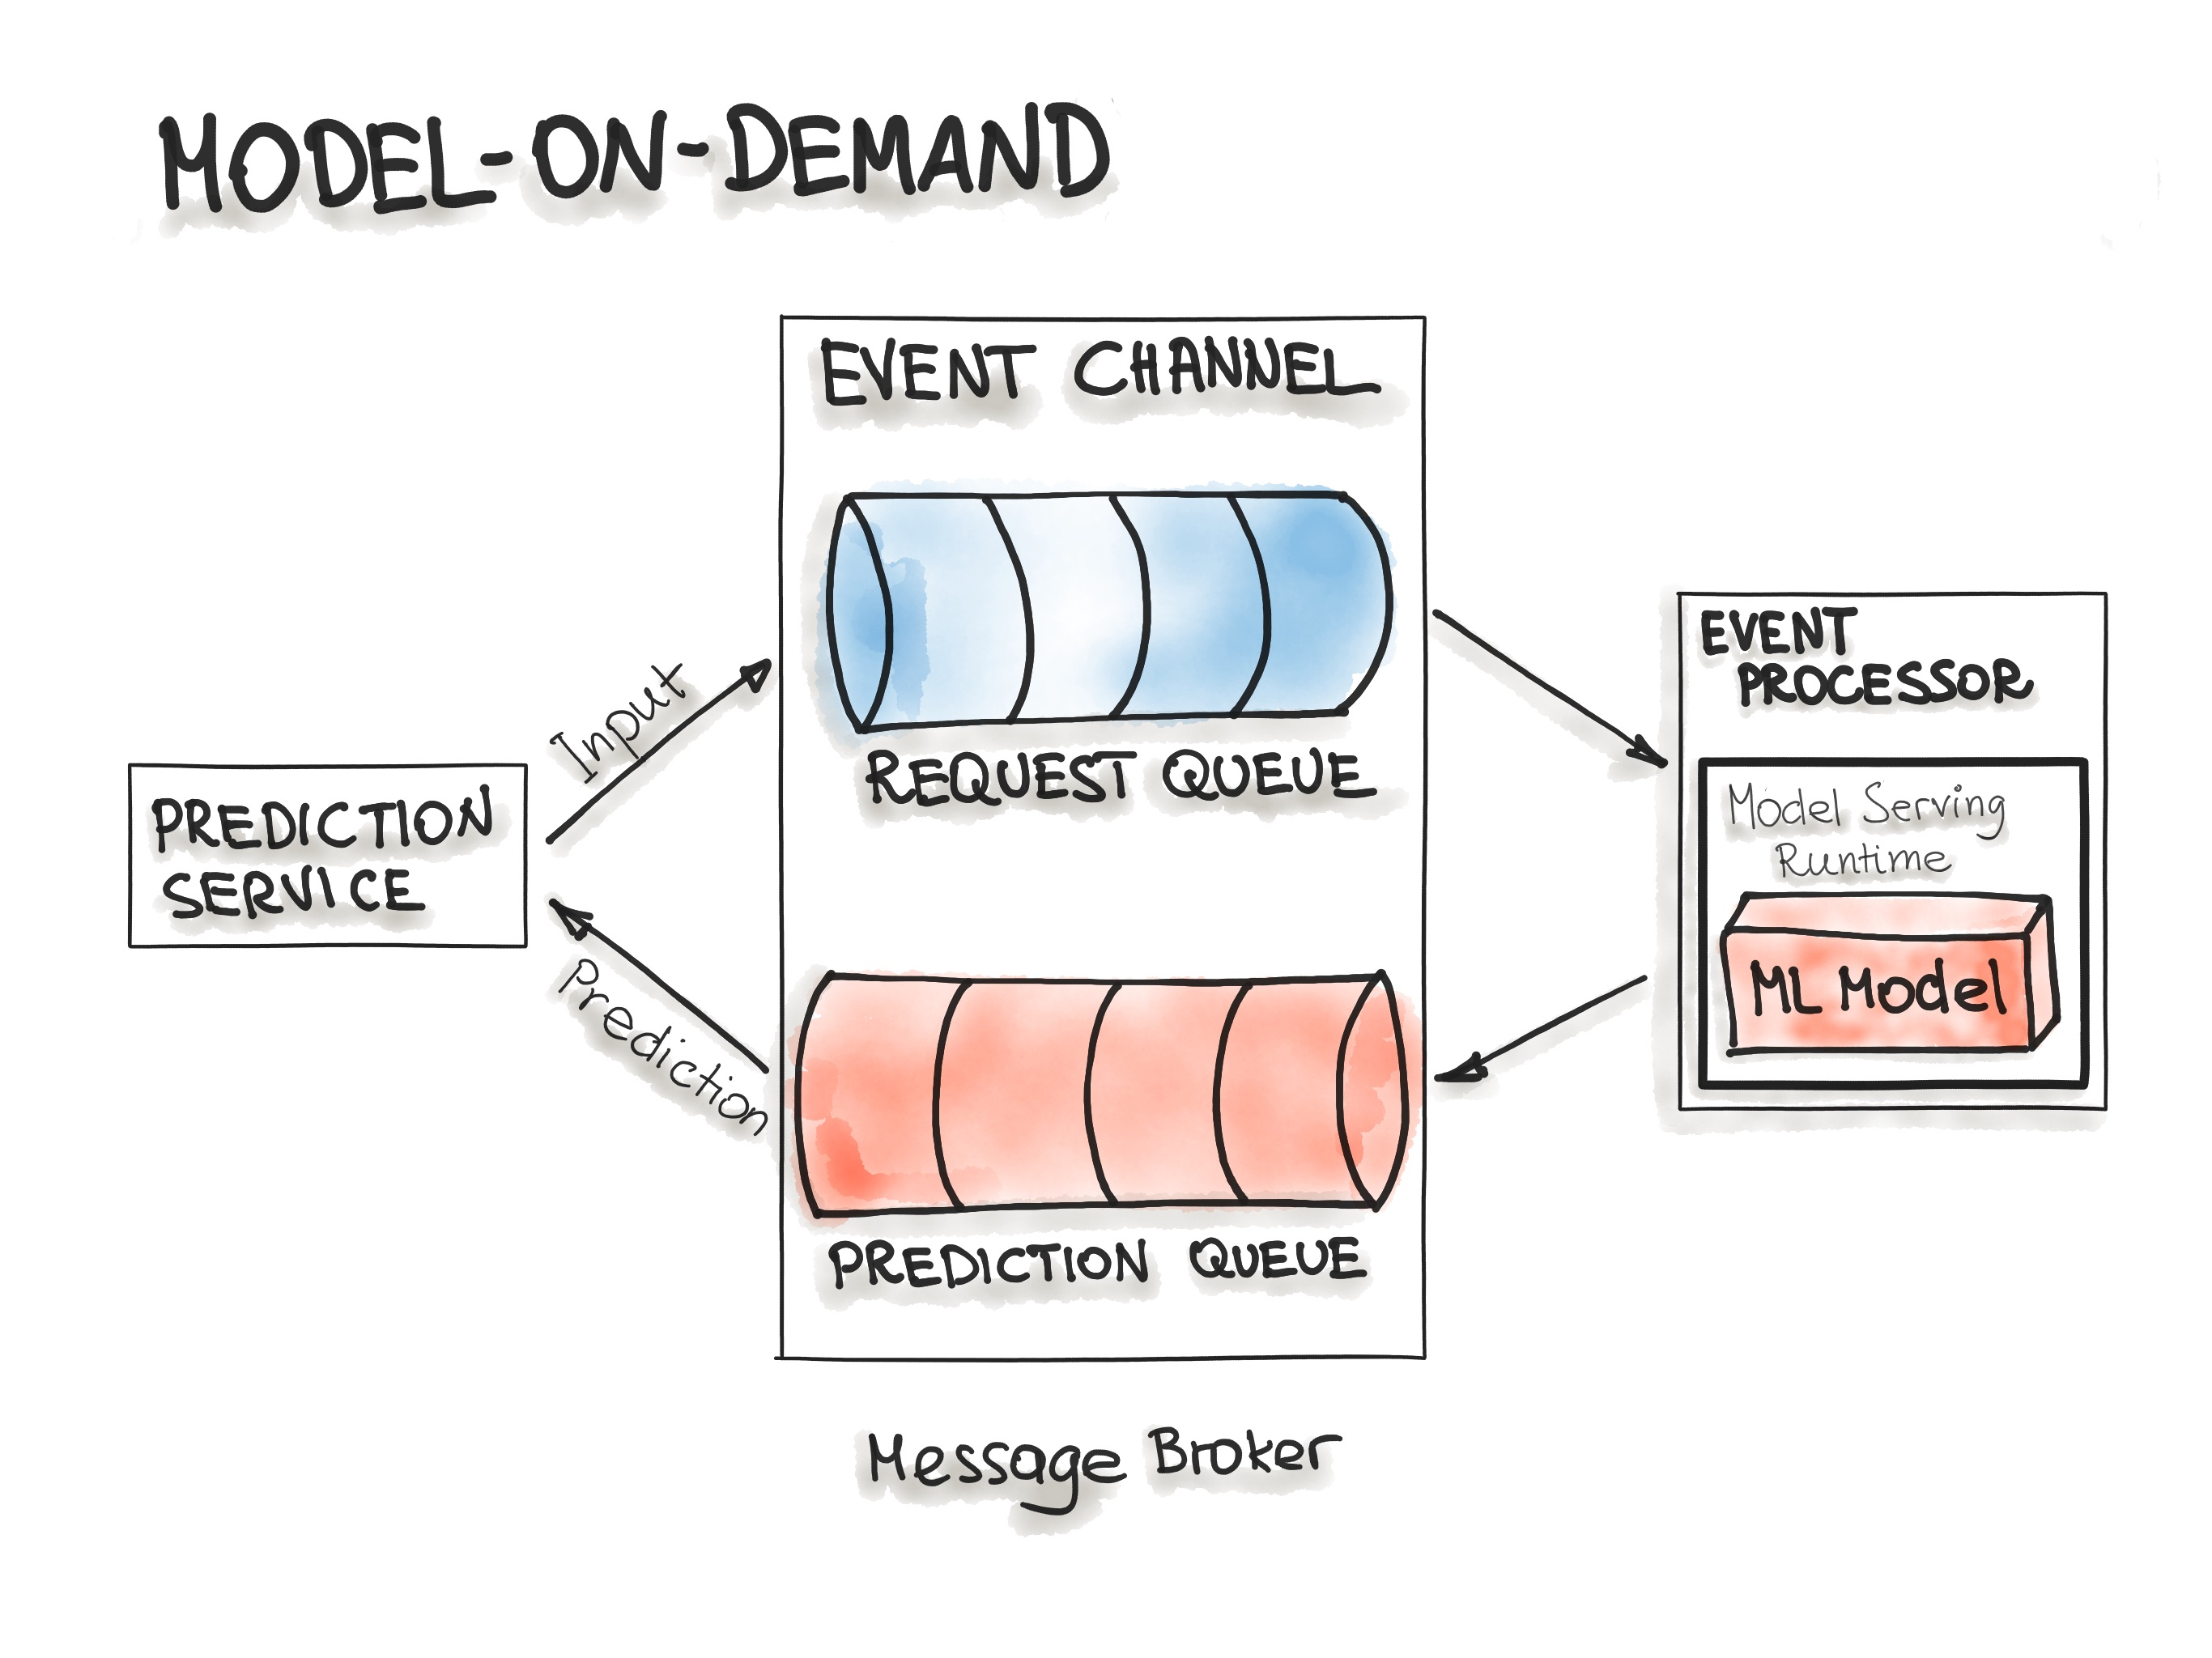
\includegraphics[width=0.7\textwidth]{02-model-on-demand.jpg}
  \caption{Ilustrasi Model-on-Demand (Sumber:~\cite{book-handsonml})}\label{fig:model-on-demand}
\end{figure}

Pada dasarnya, \textit{pattern} ini memiliki karakteristik yang serupa dengan Model-as-Service dengan perbedaan dalam infrastruktur pembentuk sistem.
Perbedaan utamanya adalah dalam Model-as-Service, \textit{request} dijalankan secara sinkron.
Dalam \textit{pattern} Model-on-Demand, terdapat penggunaan broker sehingga request terhadap model dapat dibuat asinkron (lihat Gambar~\ref{fig:model-on-demand}).
Waktu prediksi juga dapat diatur lewat broker atau model yang digunakan.

\subsection{Hybrid Serving}

\begin{figure}[ht]
  \centering
  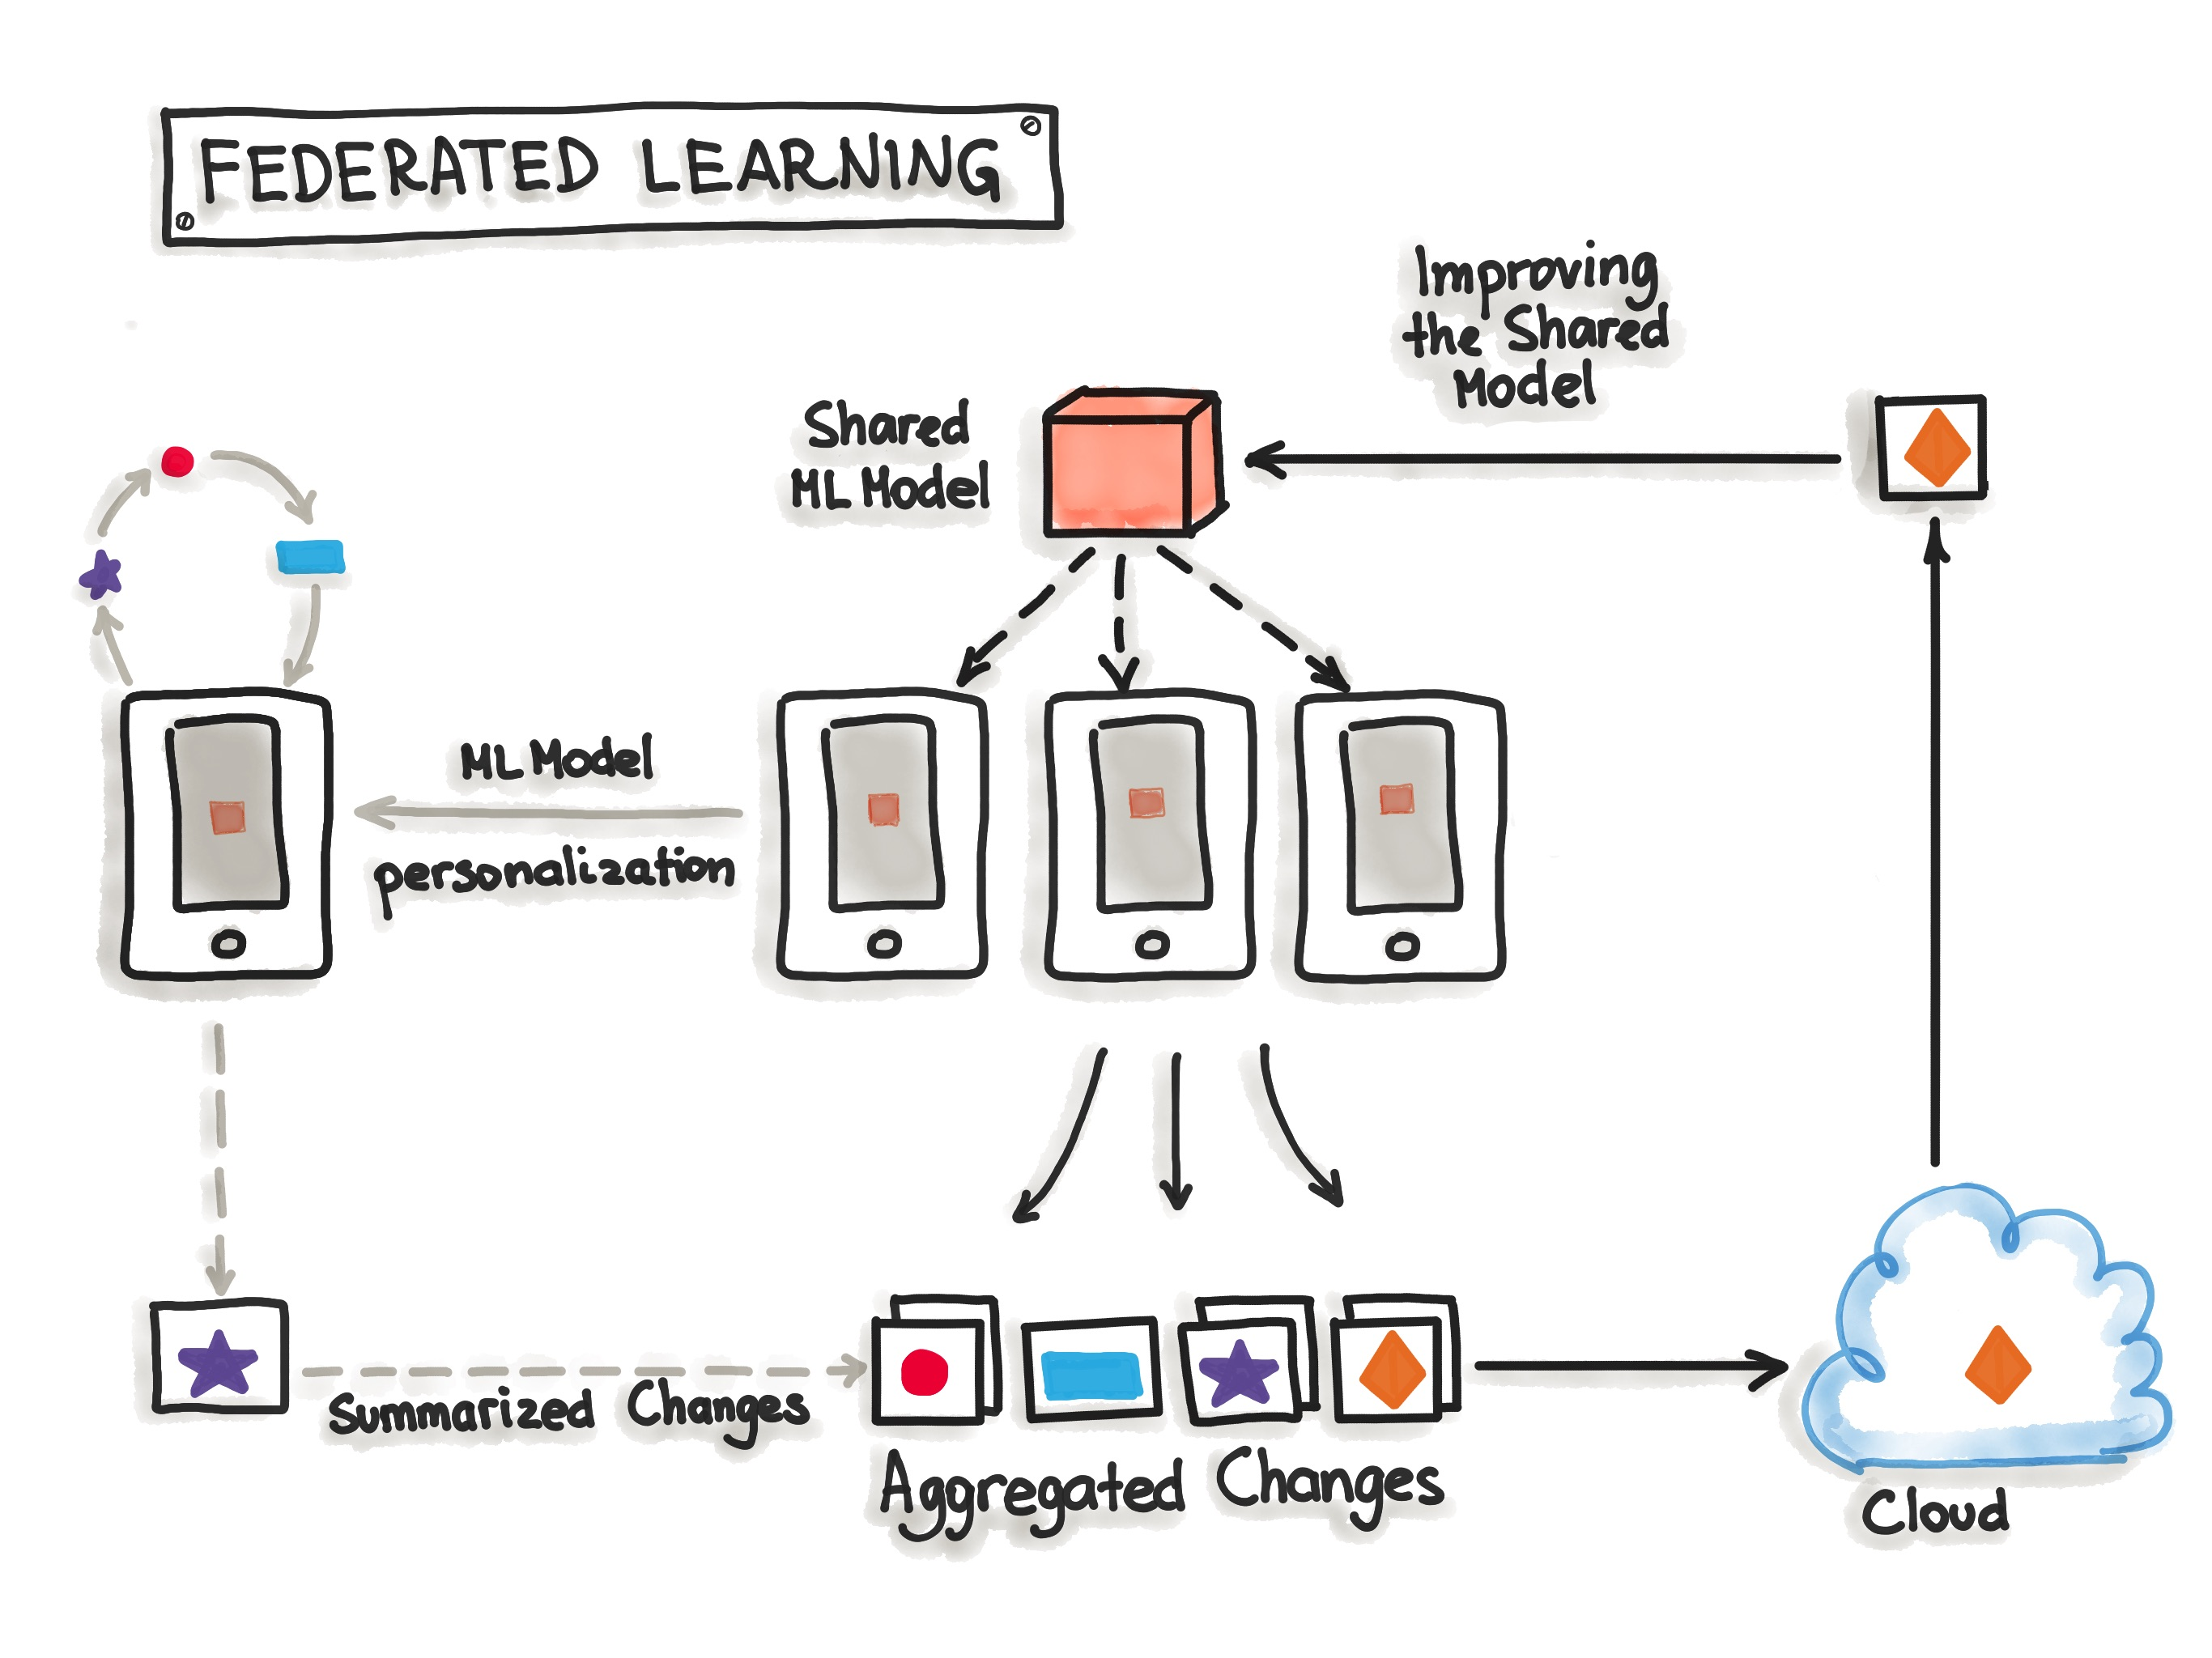
\includegraphics[width=0.7\textwidth]{02-federated-learning.jpg}
  \caption{Ilustrasi Federated Learning (Sumber:~\cite{book-handsonml})}\label{fig:federated-learning}
\end{figure}

Hybrid Serving, atau biasa dikenal dengan istilah Federated Learning, adalah teknik yang memanfaatkan beberapa perangkat untuk proses \textit{training}-nya.
Tidak hanya melakukan \textit{training} secara terpusat, model yang sudah jadi akan didistribusikan pada perangkat-perangkat berbeda.
Dari sana data pelatihan baru akan dikumpulkan dari perangkat-perangkat tersebut (lihat Gambar~\ref{fig:federated-learning}).
Data yang dikumpulkan akan dikirim ke sebuah pusat penyimpanan data untuk membuat model yang lebih mutakhir.
